\documentclass[border=0pt]{standalone}
\usepackage{tikz}
\usepackage{amsmath}
\usetikzlibrary{arrows.meta}

% ---------------------------------------------------------------
% Top view (vista dall'alto) of the thrust test bench.
%
% Layout (left to right):
%   Motor + propeller  --[arm, length ell]-->  Torquemeter -- Column
%
% The propeller axis is along X (arm direction).
% The thrust force f acts in the +Y direction (orthogonal to the arm),
% creating a torque  tau = f * ell  around the vertical axis (Z),
% which is measured by the torquemeter on the right.
% ---------------------------------------------------------------

\begin{document}
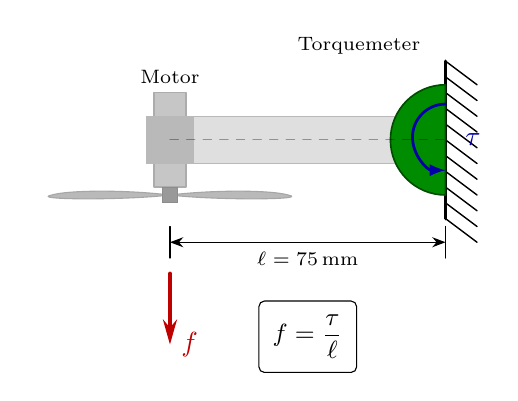
\begin{tikzpicture}[
    >=Stealth,
    line join=round,
    line cap=round,
    every node/.style={font=\small},
]

% ---------------------------------------------------------------
% Colour palette
% ---------------------------------------------------------------
\colorlet{colAlum}   {gray!30}
\colorlet{colAlumD}  {gray!55}
\colorlet{colTq}     {green!55!black}
\colorlet{colTqD}    {green!30!black}
\colorlet{colMotor}  {gray!45}
\colorlet{colMotorD} {gray!65}
\colorlet{colArm}    {gray!25}
\colorlet{colForce}  {red!75!black}
\colorlet{colTorque} {blue!65!black}
\colorlet{colOmega}  {blue!65!black}

% ---------------------------------------------------------------
% Parameters
% ---------------------------------------------------------------
\def\armLen{3.5}    % arm length (cm, represents ell)
\def\armW{0.30}     % arm half-width
\def\motorW{0.4}    % motor box width  (along X = arm direction)
\def\motorH{1.2}      % motor box height (along Y)
\def\tqR{0.7}      % torquemeter radius
\def\colW{1.4}      % column box width
\def\colH{1.0}      % column box height
\def\bladeLen{0.7}  % propeller blade half-length (along X)
\def\propOffset{-0.7} % quanto scendere sotto il motore
\def\hubSize{0.1}
\def\wallX{\armLen}  % bordo destro del torquemetro + gap
% ---------------------------------------------------------------
% Coordinate origins
%   motor centre:      (0, 0)
%   arm goes from x=0 to x=armLen
%   torquemeter centre: (armLen, 0)
%   column to the right of torquemeter
% ---------------------------------------------------------------

% -------  ARM  -----------------------------------------------
\fill[colArm, draw=colAlumD, line width=0.4pt]
    (0, -\armW) rectangle (\armLen, \armW);

% -------  MOTOR BOX  -----------------------------------------
\fill[colMotor, draw=colMotorD, line width=0.6pt, rounded corners=0pt]
    (-\motorW/2, -\motorH/2) rectangle (\motorW/2, \motorH/2);
\node[font=\scriptsize] at (0, 0.8) {Motor};

% -------  MOTOR HOLDER (bracket a U che abbraccia il motore) --
\fill[colAlumD, draw=colAlumD, line width=0.5pt]
    (-\motorW/2 - 0.1, -\armW) rectangle (\motorW/2 + 0.1, \armW);


% % -------  PROPELLER (shifted downward) ------------------------
% % blade 1: toward -X
% \draw[gray!60, line width=3pt, line cap=round, opacity=0.7]
%     (0, \propOffset) -- (-\motorW/2 - \bladeLen, \propOffset);

% % blade 2: toward +X
% \draw[gray!50, line width=3pt, line cap=round, opacity=0.7]
%     (0, \propOffset) -- (\motorW/2 + \bladeLen, \propOffset);

% \filldraw[gray!65, draw=gray!80, line width=0.4pt]
%     (-\hubSize, \propOffset - \hubSize) rectangle (\hubSize, \propOffset + \hubSize);


% % -------  PROPELLER realistica (vista dall'alto, profilo alare) --------

% Pala sinistra
\fill[gray!55, draw=gray!70, line width=0.4pt]
    (0, \propOffset)
    .. controls (-0.6, \propOffset - 0.07) and (-1.8, \propOffset - 0.06) ..
    (-1.5, \propOffset)
    .. controls (-1.3, \propOffset + 0.06) and (-0.6, \propOffset + 0.07) ..
    cycle;

% Pala destra
\fill[gray!55, draw=gray!70, line width=0.4pt]
    (0, \propOffset)
    .. controls (0.6, \propOffset - 0.07) and (1.8, \propOffset - 0.06) ..
    (1.5, \propOffset)
    .. controls (1.3, \propOffset + 0.06) and (0.6, \propOffset + 0.07) ..
    cycle;

% Albero motore / dado centrale
\fill[gray!80, draw=gray!90, line width=0.4pt]
    (-0.1, \propOffset - 0.1) rectangle (0.1, \propOffset + 0.1);

    % -------  PROPELLER — profilo visto dall'alto ----------------
% Vista dall'alto: la pala ruota nel piano XY → si vede il profilo
% di taglio (chord lungo Y, span lungo X).
% Il bordo d'attacco è più spesso, bordo di uscita sottile.

% Pala sinistra (verso -X)
% \fill[gray!55, draw=gray!70, line width=0.4pt]
%     (-\motorW/2, \propOffset + 0.15)   % bordo attacco (spesso)
%     .. controls (-0.8, \propOffset + 0.13) and (-1.4, \propOffset + 0.07) ..
%     (-1.5, \propOffset)                 % punta (sottile)
%     .. controls (-1.4, \propOffset - 0.04) and (-0.8, \propOffset - 0.05) ..
%     (-\motorW/2, \propOffset - 0.05)   % bordo uscita
%     -- cycle;

% % Pala destra (verso +X) — simmetrica
% \fill[gray!55, draw=gray!70, line width=0.4pt]
%     (\motorW/2, \propOffset + 0.13)
%     .. controls (0.8, \propOffset + 0.13) and (1.5, \propOffset + 0.07) ..
%     (1.5, \propOffset)
%     .. controls (1.4, \propOffset - 0.04) and (0.8, \propOffset - 0.05) ..
%     (\motorW/2, \propOffset - 0.05)
%     -- cycle;

% % Albero motore
% \fill[gray!80, draw=gray!90, line width=0.4pt]
%     (-0.1, \propOffset - 0.1) rectangle (0.1, \propOffset + 0.1);
    
% rotation arc (omega) — arc in XY plane around propeller axis
% \draw[-{Stealth}, colOmega, line width=0.8pt]
%     (0, -1)
%     arc[start angle=115, end angle=45, radius=0.62];
% \node[colOmega, font=\small] at (1.9, -0.7) {$\omega$};


% -------  THRUST FORCE  f  (orthogonal to arm, +Y direction) --
\draw[-{Stealth[length=9pt,width=5pt]}, colForce, line width=1.6pt]
    (0, \motorH/2 - 2.3) -- (0, -\motorH/2 - 2)
    node[right, font=\normalsize] {$f$};



% -------  WALL CONSTRAINT (vincolo a parete, lato destro torquemetro) ----
% Linea verticale della parete
\draw[line width=1.2pt]
    (\wallX, -1) -- (\wallX, 1);

% Trattini obliqui (hatching) — simbolo classico vincolo fisso
\foreach \y in {-1, -0.8, -0.6, -0.4, -0.2, 0.0, 0.2, 0.4, 0.6, 0.8,1}{
    \draw[line width=0.5pt]
        (\wallX, \y) -- (\wallX + 0.4, \y - 0.3);
}
    
% % -------  TORQUEMETER  (green circle on right end of arm) -----
% \filldraw[colTq, draw=colTqD, line width=0.6pt]
%     (\armLen, 0) circle (\tqR);

% % Label "Torquemeter" sopra
% \node[font=\scriptsize, align=center] at (\armLen, \tqR + 0.5)
%     {Torquemeter};

% % Arco tau DENTRO al cerchio
% \draw[-latex, colTorque, line width=1.0pt]
%     (\armLen + \tqR*0.55, \tqR*0.55)
%     arc[start angle=45, end angle=320, radius=\tqR*0.70];
% \node[colTorque, font=\normalsize] at (\armLen, \tqR*0.35) {$\tau$};

% Torquemetro = SEMICERCHIO (aperto a destra, lato braccio)
\filldraw[colTq, draw=colTqD, line width=0.6pt]
    (\armLen, \tqR) arc[start angle=90, end angle=270, radius=\tqR]
    -- cycle;

% Diametro verticale
\draw[colTqD, line width=0.6pt]
    (\armLen, -\tqR) -- (\armLen, \tqR);

% Etichetta
\node[font=\scriptsize, align=center] at (\armLen - \tqR - 0.4, \tqR + 0.5)
    {Torquemeter};

% Arco tau interno
\draw[-latex, colTorque, line width=1.0pt]
    (\armLen, \tqR*0.65)
    arc[start angle=90, end angle=270, radius=\tqR*0.60];

\node[colTorque, font=\normalsize] at (\armLen + \tqR/2, 0) {$\tau$};

% -------  DIMENSION LINE  ell  --------------------------------
% from motor centre to torquemeter centre, below the arm
\draw[<->, thin, ]
    (0, -\armW - 1) -- (\armLen, -\armW - 1)
    node[midway, below, font=\scriptsize, ] {$\ell = 75\,\text{mm}$};
% tick marks
\draw[thin, ]
    (0, -\armW - 0.8) -- (0, -\armW - 1.2);
\draw[thin, ]
    (\armLen, -\armW - 0.8) -- (\armLen, -\armW - 1.2);

% -------  FORMULA  -------------------------------------------
\node[draw, fill=white, rounded corners=2pt,
      font=\small, inner sep=5pt]
    at (\armLen/2, -2.5)
    {$f = \dfrac{\tau}{\ell}$};

% -------  MOMENT ARM dashed line  ----------------------------
\draw[black, dashed, opacity=0.35, thin]
    (0, 0) -- (\armLen, 0);

\end{tikzpicture}
\end{document}